\documentclass[11pt,article,oneside]{article}

\usepackage[final,nonatbib]{neurips_2024}

% Colors
\usepackage[dvipsnames]{xcolor}

% ===============
% Hyperlink setup
% ===============
\usepackage{xurl}
\usepackage[
    colorlinks,
    breaklinks=true,
    urlcolor=NavyBlue,
    citecolor=NavyBlue,
    linkcolor=NavyBlue,
    linktocpage,
]{hyperref}
\def\sectionautorefname{\S}
\def\subsectionautorefname{\S}

\usepackage{algorithm}
\usepackage{algpseudocode}
\usepackage{graphicx}
\usepackage{caption}

% Nicer monospace font
\usepackage{inconsolata}

% Using Palatino for text and math
\usepackage{newpxtext}
\usepackage{newpxmath}

% Improved typography
\usepackage{microtype}

% Bibliography setup
\usepackage[
    natbib,
    style=numeric-comp,
    sorting=none,
    doi=false,
    isbn=false,
    url=true,
    eprint=false,
    maxbibnames=10,
    hyperref
]{biblatex}
\addbibresource{bibliography.bib}
\renewcommand\bibfont{\small}
\newbibmacro{string+doiurlisbn}[1]{%
  \iffieldundef{doi}{%
    \iffieldundef{url}{%
      \iffieldundef{isbn}{%
        \iffieldundef{issn}{%
          #1%
        }{%
          \href{http://books.google.com/books?vid=ISSN\thefield{issn}}{#1}%
        }%
      }{%
        \href{http://books.google.com/books?vid=ISBN\thefield{isbn}}{#1}%
      }%
    }{%
      \href{\thefield{url}}{#1}%
    }%
  }{%
    \href{http://dx.doi.org/\thefield{doi}}{#1}%
  }%
}

\DeclareFieldFormat[article,book,incollection,inproceedings,data]{title}%
    {\usebibmacro{string+doiurlisbn}{#1}}

\DeclareFieldFormat*{url}{}
\DeclareFieldFormat[online]{url}{\mkbibacro{URL}\addcolon\space\url{#1}}

\DeclareFieldFormat[misc]{title}{\usebibmacro{string+doiurlisbn}{\mkbibemph{#1}}}


\title{Formula 1 Forecast: Predicting Formula 1 Race Results with Machine Learning}
\author{%
    Mohit Rakesh Taparia\\
    School of Information \\
    University of Arizona\\
    \texttt{mohittaparia@arizona.edu}
}
\begin{document}
\maketitle

\section{Introduction}
In the high-stakes universe of Formula One racing, every second is crucial. It is a highly esteemed and challenging motorsport that captivates millions of enthusiasts worldwide \citep{ref1}. Predicting the victory for the next season of Grand Prix is very demanding and depends upon multiple factors that come into play. Previously, when trying to predict the winner based on subjective viewpoints rather than using a data-driven methodology has not yielded accurate results. In this project, we utilize a machine learning framework and technique to predicting the upcoming Formula 1 Grand Prix race winners in each race. The model uses various factors such as weather conditions, driver and constructor standings, qualifying outcomes, race history, and more to make precise predictions. By analysing and applying regression and classification techniques the aim is to achieve accurate predictions.

Utilizing machine learning to leverage a wide array of contemporary and historical factors to predict the victor of the subsequent Grand Prix races in every season, leveraging publicly available data and datasets that is used in this project. It contains data from year 1950 to 2023 \citep{ref3}, sourced from Ergast website and Formula 1 official webpage. This dataset contains a plethora of information regarding Formula 1 races, lap times, driver IDs, positions during races, circuit characteristics, weather conditions, and historical race results. Additionally, it provides a detailed record of finishing time, incidents, and race outcomes.

To implement machine learning techniques and models to predict the winner by deploying Random Forest classification model, renowned for its effectiveness in handling structured data. Now conduct feature engineering to extract meaningful insights by identifying key features like driver standings, constructor standings, incident histories, and circuit characteristics. Then dataset preparation involves careful splitting into training, validation, and testing sets while preserving temporal aspects and normalization. We evaluate model performance using metrics like accuracy, precision, recall, and F1-score, fine-tuning hyperparameters to optimize performance and prevent overfitting\citep{ref2}.

The aim is to develop a predictive model that can assist teams in optimizing race strategy and decision-making during Formula One races. Through iterative refinement and experimentation, we strive to build a robust and reliable winner prediction system that helps examine team performance and winners in the fast-paced world of Formula One racing.
\clearpage

\section{Methods}
\subsection{Describing the Dataset}
The dataset used in this study is scraped from Ergast website \citep{ref3} and Formula 1 official website which comprises the historical Formula 1 race results and other information of past 70 years. It includes various features such as starting position, driver ID, max pace, mean pace, driver experience in races, and driver experience in years. The data is stored in csv file format and is run through different data cleaning steps to obtain final dataset. 

\subsection{Describing the Algorithm}
Random Forest Classifier algorithm is used in predicting the winners. This algorithm works on the principle of ensemble learning  which combines multiple classifier to improve the overall performance. This works by building a collection of decision trees trained on random subsets of data and features\citep{ref4}. While predicting the result, each tree is independently used, and the final prediction is determined by averaging across all trees. 
Random Forest Classifier enhances predictive accuracy and reduces overfitting, making it effective for handling multiple tasks across different features. This averaging of results helps the algorithm to improve its performance and predictions.

The training of Random Forest Classifier model is done by preparing the dataset with features and target values and splitting it into training, validation, and testing sets. This process involves creating bootstrap samples for each trees and randomly selecting features at each node by building forest of decision trees and then aggregating their predictions to get final prediction.
 

The pseudocode for a Random Forest Regression algorithm \citep{ref4} is given below:
\begin{algorithm}
    \caption{RandomForest}
    \textbf{Precondition:} A training set $S = \{(x_1,y_1), \ldots, (x_n,y_n)\}$, features $F$, and number of trees in forest $B$.
    \begin{algorithmic}[1]
    \Function{RandomForest}{$S, F, B$}
        \State $H \gets \emptyset$
        \For{$i = 1, \dots, B$}
            \State $S_i \gets$ A bootstrap sample from $S$
            \State $h_i \gets \textproc{RandomizedTreeLearn}(S_i, F)$
            \State $H \gets H \cup \{h_i\}$
        \EndFor
        \State \textbf{return} $H$
    \EndFunction
    \Function{RandomizedTreeLearn}{$S, F$}
        \State \textbf{At each node:}
        \State $f \gets$ a very small subset of $F$
        \State Split on the best feature in $f$
        \State \textbf{return} the learned tree
    \EndFunction
    \end{algorithmic}
\end{algorithm}




\subsection{Evaluation Procedure}
Once the model is trained using training data a custom function "point Classifier" is created and used to evaluate each trained model \citep{ref5}. The custom function check the precision score for each model and each race in the test season and average the scores to find the overall performance of the model and then rank then based on their performance score.
Now the best evaluated model is selected and fitted in training data. Then Principle Component Analysis (PCM) \citep{ref6} which is an unsupervised learning algorithm technique used to examine the relation among variables. When applying PCA on Random Forest Classifier it can help improve model performance and speed up training as it allows to choose desired number of variables for training the model.


\subsection{Hyperparameter Tuning}
Hyperparameter tuning is an important step in optimizing the performance of machine learning models \citep{ref7}. In this project, hyperparameter tuning is applied after running grid search algorithm which finds that best possible hyperparameter values. It uses combination of each hyperparameter in the grid and train the model by evaluating the performance using cross-validation.
This is repeated to find the combination of hyperparameters with best results for the model.

\begin{verbatim}
    'criterion': ['gini', 'entropy']
    'max_features':['sqrt', 'log2', None]
    'max_depth': [5, 55, 20] 
\end{verbatim}

\section{Results}
\subsection{Correlation Analysis}
Finding correlation between the features and target variable of the data is the most crucial step as it help in training the model to predict results accurately \citep{ref8}. To analyse the correlation by creating an correlation matrix from the dataset which is then used to plot a heat-map. The plotted map highlight the best relationship driver wins, constructor wins and other variables. 
From the plot we can say that constructor wins an driver points have maximum correlation.

\begin{figure}[htbp]
    \centering
    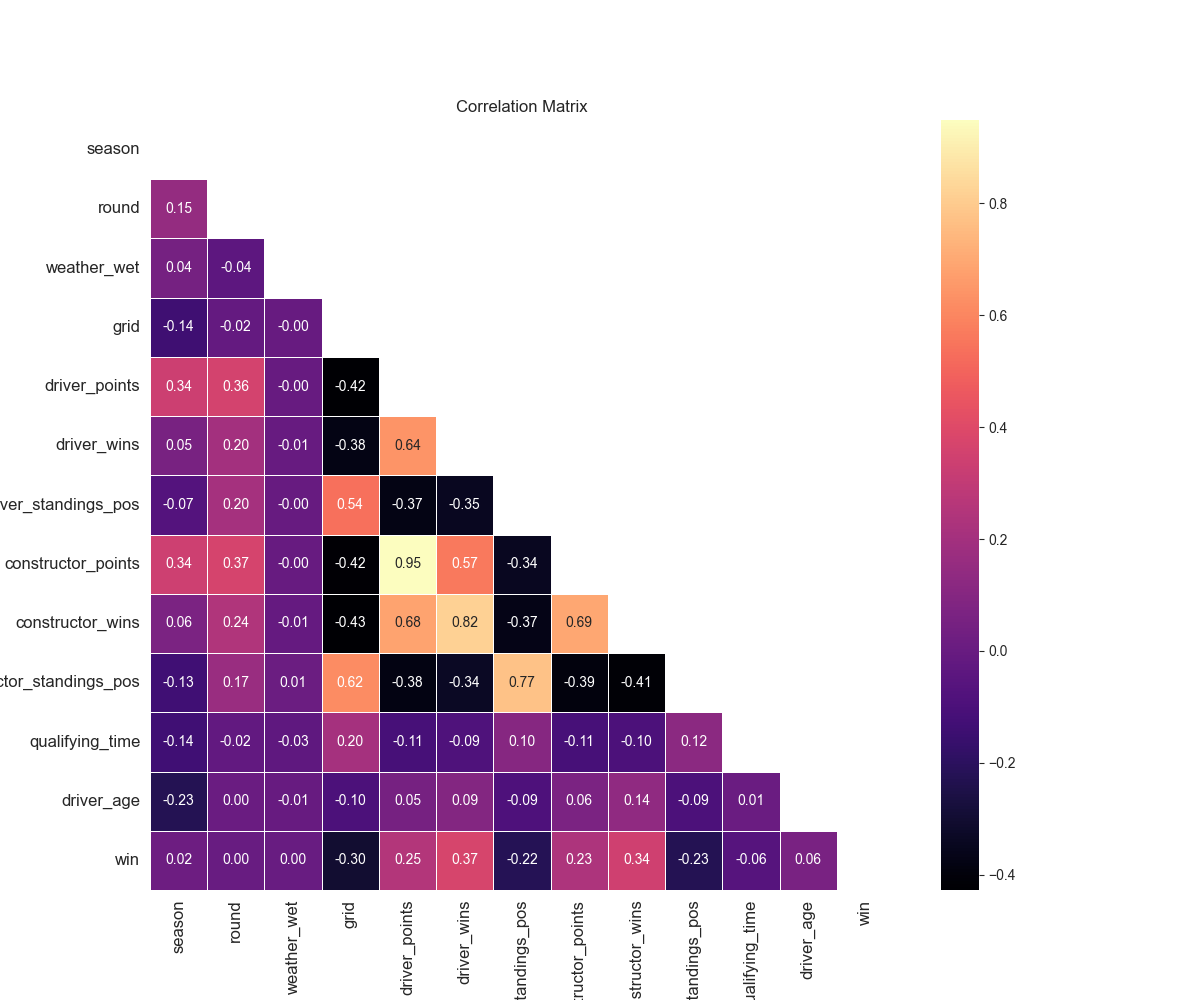
\includegraphics[width=0.8\textwidth]{code/Images/correlation_heat-map.png}
    \caption{Correlation features Heat-map}
\end{figure}

Now after analysing the heat-map a side-by-side box plot is plotted which check if the values actually correlate for constructor wins and other features like driver points, driver wins, driver standings pos, constructor points, constructor standings pos, qualifying time, and driver age.

\begin{figure}[htbp]
    \centering
    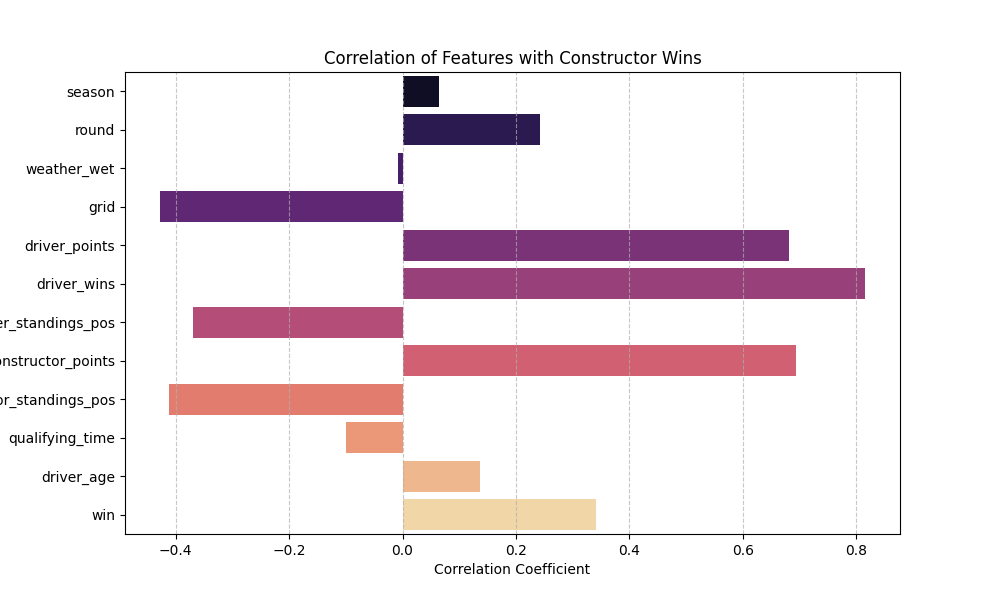
\includegraphics[width=0.9\textwidth]{code/Images/constructor_wins_correlation_plot.png}
    \caption{Box plot to find Correlation between constructor wins and other features}
\end{figure}
 
Based on the plot some features like driver points, driver wins, constructor points have positive correlation with constructor wins which means that if the values of those features increase chances of constructor wins also incresase.
Now opposite is analysed for all the other features which can lower the chances of wins. So based on this the model is trained with positive features as it has high correlation with target value. 

\subsection{Model Performance}
Based on the above findings the selected model is used to make prediction on the test data. To check model performance classification metrix such as accuracy score, confusion matrix and classification report is generate and the results are given below. 

Test Accuracy: 0.959 \\
Cross-Validation Scores: [0.959, 0.957, 0.954, 0.957, 0.955] \\
Mean CV Score: 0.956 \\

\begin{table}[H]
    \centering
    \caption{Classification Report}
    \label{tab:best_model_classification_report}
    \begin{tabular}{|l|l|l|l|l|}
    \hline
    \textbf{Class}  & \textbf{Precision} & \textbf{Recall} & \textbf{F1-Score} & \textbf{Support}  \\ \hline
    0               & 0.95              & 1.00             & 0.97              & 280                  \\ \hline
    1               & 0.00              & 0.00             & 0.00              & 15                   \\ \hline
    Accuracy        & \multicolumn{3}{c}{\hspace{3cm} 0.95}                    & 295                  \\ \hline
    Macro Avg       & 0.47              & 0.50             & 0.49              & 295                   \\ \hline
    Weighted Avg    & 0.90              & 0.95             & 0.92              & 295                   \\ \hline
    \end{tabular}
\end{table}

\begin{figure}[htbp]
    \centering
    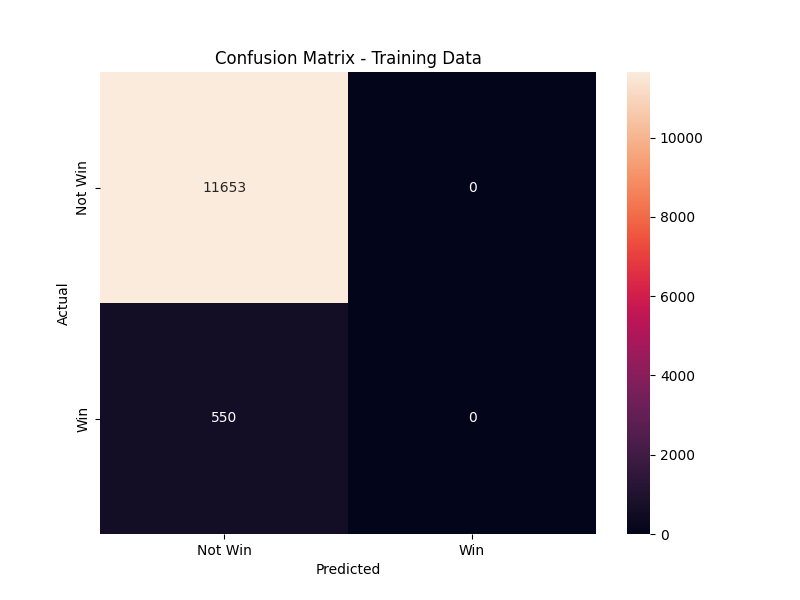
\includegraphics[width=0.9\textwidth]{code/Images/confusion_matrix.png}
    \caption{Confusion Matrix for Traning Data}
\end{figure}

Prediction total, accuracy and Percentage of success for Random Forest Classification is given below. The result shown suggest that the model is overfitting the training data so to overcome this further analysis is required.

Results for Random Forest Classifier:\\
Accuracy Score: 0.9491525423728814\\
Total Correct Predictions: 280 / 295\\
Percent Success: 94.92\%\\

\subsection{Prediction}   
When training the Random Forest Classifier Model with data from 2021 season to predict the winners of that season which shows that the model is 95 \% accurate. The predicted result is shown in the table below. From the table it can be seen that driver Hamilton and constructor Mercedes has won most of the races in the year 2021. 
He was awarded best driver award and also team received best constructor award for 2020.

\begin{table}[htbp]
    \centering
    \caption{Predicted Winners for the Year 2021}
    \label{tab:predicted_mvp_shares}
    \begin{tabular}{|l|l|l|l|l|l|}
    \hline
    \textbf{Season}  & \textbf{Round}  & \textbf{Driver won} & \textbf{Driver Prediction} & \textbf{Constructor won} &\textbf{Constructor Predicted} \\ \hline
    2021             & 1              & Bottas              & Verstappen                  & mercedes                 & ferrari                       \\ \hline
    2021             & 2              & Hamilton            & Hamilton                    & mercedes                 & alpine                        \\ \hline
    2021             & 3              & hamilton            & hamilton                    & mercedes                 & mercedes                         \\ \hline
    2021             & 4              & hamilton            & hamilton                    & mercedes                 & alpine                          \\ \hline
    2021             & 5              & verstappen          & hamilton                    & red bull                 & mercedes                           \\ \hline
    2021             & 6              & hamilton            & hamilton                    & mercedes                 & mercedes                            \\ \hline
    2021             & 7              & hamilton            & hamilton                    & mercedes                 & mercedes                             \\ \hline
    2021             & 8              & gasly               & hamilton                    & alphatauri                 & mercedes                              \\ \hline
    2021             & 9              & hamilton            & hamilton                    & mercedes                 & mercedes                               \\ \hline
    2021             & 10             & bottas              & hamilton                    & mercedes                 & mercedes                                \\ \hline
    2021             & 11             & hamilton            & hamilton                    & mercedes                 & mercedes                                 \\ \hline
    2021             & 12             & hamilton            & hamilton                    & mercedes                 & mercedes                                  \\ \hline
    2021             & 13             & hamilton            & bottas                      & mercedes                 & mercedes                                  \\ \hline
    2021             & 14             & hamilton            & hamilton                    & mercedes                 & mercedes                                  \\ \hline
    2021             & 15             & hamilton            & russell                    & mercedes                 & williams                                  \\ \hline
    2021             & 16             & hamilton            & vettel                    & mercedes                 & ferrari                                \\ \hline
    2021             & 17             & verstappen          & hamilton                    & red bull                 & mercedes                                 \\ \hline
    
    \end{tabular}
\end{table}

\section{Discussion}

The project presents a robust framework for predicting Formula One race winners using machine learning techniques, specifically Random Forest Classification by considering a wind range of historic data spanning from 1950 to 2022. The model aims to provide accurate predictions which can assist teams in optimizing race strategy and decision making while racing.
Future improvements, like modifying the existing model by optimizing hyperparameter tuning and comparing it with different models to get better prediction accuracy. Also, implementing this model as an webapp for public usage can significantly help in improving this project. 


In conclusion, while this project shows predictions for the year 2020 with an accuracy of 94\% which is due to overfitting. However, New regulations and changes in Formula 1 racing may impact the models future predictions. 
Overall, this project have achieved an significant accuracy in predicting winners which shows the potential of Machine learning in field of motorsports that has sets a stage for further research and development in this area to improve the race predictions.

\printbibliography

\end{document}
